In this study, we investigated the sex and mass effects on three musculoskeletal indicators when women and men lifted 6~kg and 12~kg boxes from hip to eye level.
As hypothesized, women generated more muscle force and activation than men, regardless of the mass lifted.
Those differences occurred during the dropping phase, when the box was above shoulder level.
In addition, women spent more time beyond a shear-compression dislocation ratio.

\subsection{General profile of muscle forces and activations}\label{subsec:general-profile-of-muscle-forces-and-activations}

As previously reported in electromyography~\cite{Bouffard2019-fd}, our results show that participants generated two distinct peaks of muscle forces and activations during the pulling and dropping phases.
Those two peaks appear when the box is the furthest from the trunk (\ref{sec:box-thorax-distance-and-hip-displacement}) leading to a longer--ineffective--lever arm which decreases the mechanical efficiency of the lift.
The second peak reached a higher force and activation amplitude, probably due to elongated muscle lever arms when participants lifted the box higher, which requires more muscle activation to stabilize the upper limb.
As the muscle force and activation increase with the box height, the risk of upper limb injury is also likely to increase~\cite{Blache2015-oc}.
A wide range of studies already pointed out that exposure to above-shoulder work contributes to degenerative damage to the rotator cuff (see \citet{Van_der_Molen2017-sb} for a review) and should be avoided.
Similarly and as expected, a heavier box generates higher musculoskeletal stresses when the box is the furthest from the trunk.
This is in accordance with the literature~\cite{Blache2015-xe, Yoon2012-ap} and our electromyographic study~\cite{Bouffard2019-fd} and suggest lifting lighter boxes to avoid \textsc{ulmd}s.

The anterior and lateral deltoids are the prime movers during box lifting tasks~\cite{Blache2017-pv,Blache2015-oc,Bouffard2019-fd}.
Our results show that these muscles are highly solicited, in terms of muscle force and activation.
In agreement with \citet{Blache2015-oc}, the upper trapezius and infraspinatus also showed high forces and activations.
These muscles participate in arm elevation~\cite{Ackland2008-vt, Escamilla2009-ho} and their contribution increases with the lifting height~\cite{Blache2015-oc, Herberts1984-xk}.
Although we expected for antagonists (e.g., posterior deltoid, triceps brachii) and stabilizing (e.g., coracobrachialis, teres major) muscles to be less activated than agonists, our results show that the contribution of these muscles is almost null.
The static optimization cost function--which minimize the sum of squared muscle activations--is well known to neglect the stabilization and coactivation components~\cite{Gottlieb2000-ga, Kian2019-gz} and could explain why half of our data points are close to zero.

\subsection{Kinematic, electromyographic and musculoskeletal evidences of the sex-related differences}\label{subsec:kinematic,-electromyographic-and-musculoskeletal-evidences-of-the-sex-related-differences}

The physiological differences between women and men are well documented (see \citet{Cote2012-hn} for a review) and result with women’s lifting strength ranging between 40 and 70\% of men’s \citet{Kumar2004-fv}.
For a given load, women are thus closer to their maximum capacity than men.
While the kinematic differences reported in \citet{Martinez2019-mm} depend on the mass lifted by women, no sex-mass interaction was reported in \citet{Bouffard2019-fd} and in this study.
For any men-women mass ratio (100\%: 6--6~kg and 12--12~kg;
50\%: 6--12~kg), women still have higher \textsc{emg}~\cite{Bouffard2019-fd}, muscle forces and muscle activations.
This suggests that, either a 50\% mass reduction is not sufficient to control for strength differences, or that strength alone does not explain the musculoskeletal differences.
If the first suggestion is proven, acceptable weights should be reviewed as it would be expected that 90\% of women would be able to safely lift a 12~kg box from hip to eye level twice every minute for an 8-hour shift~\cite{Waters1993-nk,Waters2016-lw}.
The second suggestion seems more plausible--while strength alone does not explain EMG and musculoskeletal differences, the kinematics adaptations in response to a different box mass-strength ratio could.
Women would compensate for their strength deficits with a safe technique, but surprisingly the opposite happens and in a different way depending on the box mass.
We showed that women use more the glenohumeral joint~\cite{Martinez2019-mm} and keep the box further from the trunk (\ref{sec:box-thorax-distance-and-hip-displacement}) to lift a 6~kg box compared to men.
In addition to increasing loading on the spine~\cite{Marras2006-jq}, this technique could also increase forces located at the shoulder joint during extreme range of motion~\cite{Kim2003-lf}.
An increase in the mass to lift can change coordination to reduce the amount of muscle effort required~\cite{Burgess-Limerick1995-uh}, but still women use their lower limbs less than men to lift a 12~kg box (\ref{sec:box-thorax-distance-and-hip-displacement}).
By taking more contribution to the box height, the use of lower limbs could reduce shoulder stress~\cite{Kim2003-lf}.
Thus, men would systematically use a safer technique than women for all the weights we considered, which could explain why women have higher musculoskeletal loads in our study.

It seems unlikely that the kinematic alterations just described do not lead to a different muscle coordination scheme.
During the experimental task, women indeed generated a higher sum of muscle activations and forces than men during the dropping phase.
\citet{Bouffard2019-fd} also reported higher muscle activation in women, particularly for prime movers.
In both studies, the muscle activation in the 90\textsuperscript{th} percentile reached by women seems to be a major muscular effort to be maintained in professional settings (around 65\% MVC in women against 50\% MVC in men).

We have also shown that women spend more time with a high risk of humerus dislocation.
A greater muscle activation, muscle force and glenohumeral contribution during the handling task will indeed increase the sollication of passive structures and alter the glenohumeral stability~\cite{Bergmann2007-zj}.
This high ratio of shear and compression forces imposes high stresses on the stabilizing muscles and thus increases the risk of developing \textsc{ulmd}.
The infraspinatus, anterior deltoid and lateral deltoid muscles are all three stabilizers of the humerus~\cite{Blache2017-pv, Yanagawa2008-es} and are also the muscles with the highest sum of muscle forces in our dataset.
This underlines the importance of strengthening those muscles for manual handling workers to maintain shoulder stability and avoid injuries~\cite{Sharkey1995-gl}.

Women generally work more often and for a longer time than men in an overhead position~\cite{Dahlberg2004-mw}.
The sex-related differences reported in our three studies occurred mainly in this position, which is considered a risk factor for shoulder injuries~\cite{Antony2010-ji, Dal_Maso2016-ol, Grieve2008-je} and the leading cause of rotator cuff tear~\cite{Palmerud2000-mp, Vecchio1995-ke}.

As a summary, our previous works in kinematics~\cite{Martinez2019-mm} and electromyography~\cite{Bouffard2019-fd} showcased sex-related differences during a box lifting task.
In this study, we found evidence of a sex effect on musculoskeletal indicators.
These three categories of indicators are, by definition, dependent on each other.
Taken together, however, they do provide an overview of the complex interaction between biomechanical variables that could explain the higher prevalence of ULMD among women (Figure~\ref{fig:links}).
This interaction starts with the biological differences mentioned in \citet{Cote2012-hn}.
Women would compensate for these biological differences by altering their lifting technique, as reported in~\cite{Martinez2019-mm}.
These kinematic differences will then influence muscle activations, reported in~\cite{Bouffard2019-fd}, and the musculoskeletal loads mentioned in this study.
Greater musculoskeletal loads--in addition to unobserved factors--may explain the higher prevalence of upper limb injury in women.

\begin{figure}[H]
    \centering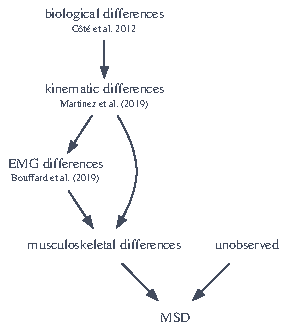
\includegraphics[width=0.5\linewidth]{fig/links.pdf}
    \caption{Conceptual framework to link the biomechanical evidences underlying the sex-related differences in the prevalence of upper limb \textsc{ulmd}.}
    \label{fig:links}
\end{figure}

\subsection{Methodological considerations}\label{subsec:methodological-considerations}

To properly interpret the results of this study, it is necessary to consider some methodological points concerning the experimental task, the scaling of the musculoskeletal model and the static optimization.
First, we designed the experimental task to control for sex effect on deposit height (shelf adjusted at eye level) and box mass (6 and 12~kg).
We showed a sex main effect regardless of the mass.
It would be preferable to measure the maximum strength of each participant and adjust the box mass accordingly to control for strength effect on our variables.
Second, many simplifying hypotheses are required when creating a musculoskeletal model, whether on muscle parameters or on muscle forces distribution to solve muscle redundancy.
One of the first limitations comes from the validation of the muscle trajectories of the \citet{Wu2016-kw} model performed on simple movements compared to our complex handling task.
In addition, the use of a generic model does not allow the musculoskeletal parameters to be personalized for each participant.
As a result, inter-individual variability is reduced and the activation or strength of certain muscles may be overestimated.
The adaptation of a musculoskeletal model to various populations and to a task above the shoulders involved many technical challenges, particularly in terms of muscle trajectories (\ref{sec:custom-wu-shoulder-model}).
Despite the above limitations, few biomechanical, ergonomic or musculoskeletal studies include so many participants from specific populations ($n = 40$).
Third, muscle forces and activations estimated from static optimization can be influenced by several factors such as the cost function, the model parameters and the joint kinematics~\cite{Bolsterlee2013-ij, Gottlieb2000-ga}.
The main limitation of our static optimization is that it does not consider muscle co-activation with a least square cost function~\cite{Kian2019-gz}.
Several solutions exist to obtain physiological activations.
The implementation of a non-dislocation constraint on the humerus~\cite{Blache2017-pv} to ensure that the balance of muscular forces is oriented towards the glenoid, the tracking of \textsc{emg} signals~\cite{Pizzolato2015-gm} or a direct dynamic approach with \textsc{emg} signals tracking~\cite{Belaise2018-wo} are some of them.
\citet{Bouffard2019-fd} have shown that sex has no effect on glenohumeral muscle co-activation, which nuances the need to include co-activation in the study of sex-related differences during a lifting task.

\subsection{Implications}\label{subsec:implications}

Work-related musculoskeletal injury is a complex multi-causal phenomenon.
Our results suggest a careful consideration of sex during ergonomic interventions on overhead tasks.
With our work on kinematics, electromyography and musculoskeletal modelling, we developed new biomechanical \textsc{ulmd} risk indicators.
The development of synthetic indicators is a step towards objective quantification of exposure to physical risk factors.
They can be used to evaluate a particular work task or technique and estimate the underlying musculoskeletal loads.
They are, for example, already applied in ergonomics investigation to report the expertise-related difference during a lifting task \cite{goubault-evsn}.
In our case, these synthetic indicators emphasized the importance of a proper lifting technique on musculoskeletal loads and by extension \textsc{ulmd} prevalence.
In order to mitigate the musculoskeletal loads on the upper limb during a lifting task, we recommend a technique that keeps the box closer from the trunk, reduces above shoulder work, makes greater use of the lower limbs and reduces the glenohumeral joint contribution.
Practitioners may also consider adapting the work environment to include lighter boxes, stabilizing muscle strengthening sessions and more generally physical activity to improve muscle strength and endurance.
These incentives are particularly recommended for female workers to compensate for the strength differential compared to men.
Beyond sex-related differences, we defend an ergonomic practice based on a process tailored to each worker and based on multidisciplinary scientific works.